\documentclass[11pt]{report}

% ============================================================
% PROJECT DOCUMENTATION TEMPLATE
% Structure based on the Sales Assist sample documentation.
% Guidance boxes flag the most common Iteration 1 pitfalls
% (see pitfalls.pdf) at the point in the document where teams
% most often make them. Delete the guidance boxes once you are
% confident a section is complete -- do not leave them in your
% final submission.
% ============================================================

\usepackage[margin=1in]{geometry}
\usepackage{titlesec}
\usepackage{fancyhdr}
\usepackage{enumitem}
\usepackage{longtable}
\usepackage{array}
\usepackage{graphicx}
\usepackage{tcolorbox}
\usepackage{hyperref}
\usepackage{xcolor}

\tcbuselibrary{skins,breakable}

% ---------- Guidance box (remove before final submission) ----------
\newtcolorbox{guidance}[1][]{
  breakable,
  colback=yellow!8,
  colframe=orange!70!black,
  fonttitle=\bfseries,
  title={Watch out: #1},
  boxrule=0.6pt,
  arc=2pt,
  left=6pt, right=6pt, top=4pt, bottom=4pt
}

% ---------- Fill-in placeholder ----------
\newcommand{\fillin}[1]{\textcolor{gray!70}{\emph{[#1]}}}

\pagestyle{fancy}
\fancyhf{}
\rhead{\thepage}
\lhead{\leftmark}
\renewcommand{\headrulewidth}{0.4pt}

\titleformat{\chapter}[hang]{\normalfont\huge\bfseries}{\thechapter.}{1em}{}
\setlist[itemize]{leftmargin=1.5em}

% ============================================================
\title{\textbf{\fillin{Project Name}\\Documentation}}
\author{
{Alejandro Garcia Jr}\\ {Garrett DeYong} \\ {Nicholas Nolen}\\ {William Waweru}\\ {Gan-Orgil Gantumur}}
\date{{9/27/2026}}

\begin{document}

\maketitle
\tableofcontents

% ============================================================
\chapter*{Change Log}
\addcontentsline{toc}{chapter}{Change Log}

\begin{guidance}[Treating early iterations as "draft"]
Do not use placeholder text or "to be decided" sections anywhere in this
document. Each iteration should be written as a complete, reviewable
deliverable -- assume it is final unless a later iteration explicitly
revises it.
\end{guidance}

\textbf{Iteration 1:}
\begin{itemize}
  \item \fillin{What was created/changed in Iteration 1}
\end{itemize}

\textbf{Iteration 2:}
\begin{itemize}
  \item \fillin{What was created/changed in Iteration 2}
\end{itemize}

\textbf{Iteration 3:}
\begin{itemize}
  \item \fillin{What was created/changed in Iteration 3}
\end{itemize}

\textbf{Final Iteration:}
\begin{itemize}
  \item \fillin{What was created/changed in the Final Iteration}
\end{itemize}

% ============================================================
\chapter{Requirements Analysis}

\begin{guidance}[Analysis before implementation]
Finish this section and the Use Cases section \emph{before} you discuss
any classes, code, or UI screens elsewhere in the document. Every
planned feature must trace to at least one requirement and one use case.
Avoid phrases like "we plan to implement \ldots" without first explaining
\emph{why} the feature is needed from the user's perspective.
\end{guidance}

\textbf{Customer / Stakeholder Perspective:}
Small independent artists need a platform to host their art and foster deeper connections with their fan communities. As an artist, I want a hybrid social media and art hosting site to upload my music, images, and stories, promote events, and interact directly with my supporters through messages and videos. As a fan, I want to discover new artists near me, follow their updates, attend their shows, and interact with other members of the community. As an administrator, I need tools to moderate the platform, review applications, and keep the community safe.

\textbf{Functional Requirements:}
\begin{itemize}
  \item The system must support role-based access control with distinct permissions and workflows for Fans, Artists, and Administrators.
  \item The system must allow Artists to maintain a profile, upload multimedia content (music, art images, stories, videos), and promote their events.
  \item The system must enable Fans to maintain an "about" profile and discover new artists using a proximity-based radius search.
  \item The system must provide a messaging infrastructure allowing fans to message artists and each other.
  \item The system must allow Administrators to review prospective artist applications, respond to user reports, and manage/ban accounts violating the Terms of Service (ToS).
\end{itemize}

\textbf{Non-Functional Requirements / Environment:}
\begin{itemize}
  \item The system must be a web-based application utilizing a 3-tier architecture (frontend web server, backend application layer, and database) to handle persistence and advanced business logic.
  \item The system must be deployed to a cloud hosting service such as Google Cloud Platform (GCP), Amazon Web Services (AWS), or Microsoft Azure.
  \item The development lifecycle must incorporate a CI/CD pipeline with mandatory pull requests.
  \item Any optional AI functionalities (e.g., content moderation, recommendation engines, or AI-generated art detectors) must be designed to respect user privacy, include human oversight, and feature fallback behavior.
\end{itemize}

\section*{Requirements Clarification Questions}
\begin{guidance}[Track open questions]
List any clarification questions your team has raised with the client
or instructor, and the answers once given. Update this list every
iteration rather than deleting resolved items -- it shows the grader
your requirements evolved deliberately.
\end{guidance}
\begin{itemize}
  \item \textbf{Q:} \fillin{Question} \\ \textbf{A:} \fillin{Answer, or "Pending"}
\end{itemize}

% ============================================================
\chapter{User Story}

\begin{guidance}[Requirements traceability]
Every requirement above should be reflected in at least one user story,
and every user story should later map to a use case. Keep IDs or
consistent wording so a reader can trace a requirement all the way
through to the System Sequence Diagrams.
\end{guidance}

\begin{itemize}
  \item As a \fillin{role}, I want to \fillin{goal} so that \fillin{benefit}.
  \item As a \fillin{role}, I want to \fillin{goal} so that \fillin{benefit}.
  \item As a \fillin{role}, I want to \fillin{goal} so that \fillin{benefit}.
\end{itemize}

% ============================================================
\chapter{Key Technical Challenges}

\begin{itemize}
  \item \fillin{Challenge 1 and how it will be approached}
  \item \fillin{Challenge 2 and how it will be approached}
\end{itemize}

\section*{Key Risks}
\begin{itemize}
  \item \fillin{Risk 1}
  \item \fillin{Risk 2}
\end{itemize}

\section*{Competition}
\begin{itemize}
  \item \fillin{Competitor / existing solution 1 -- what it does, what it lacks}
  \item \fillin{Competitor / existing solution 2}
\end{itemize}

% ============================================================
\chapter{What's New?}

\fillin{Summarize what is novel about this project compared to
existing solutions listed under Competition.}

% ============================================================
\chapter{Workflow}

\begin{guidance}[System boundary]
Make sure the workflow diagram clearly separates what the \emph{actor}
does from what the \emph{system} does. Actors should never be shown
performing system responsibilities (e.g., "system authenticates," not
"user authenticates"), and external systems should not be drawn as if
they were internal components.
\end{guidance}

\fillin{Insert workflow / activity diagram here, e.g.\\
\texttt{\textbackslash includegraphics[width=\textbackslash textwidth]\{workflow.png\}}}

% ============================================================
\chapter{Use Cases}

\begin{guidance}[Use cases are not UI click-throughs]
Do not write use cases as a sequence of UI actions ("user clicks
button, system shows page"). Describe the \emph{system's
responsibilities and guarantees} -- business rules, alternative flows,
and constraints -- not screen navigation. UI details will change over
time; system behavior should be the stable part of the documentation.
\end{guidance}

\begin{guidance}[Fully-dressed format required]
Each team member is responsible for exactly 3 use cases in
\emph{fully-dressed} form (Primary Actor, Preconditions, Postconditions,
Main Success Scenario, Extensions). A one-line summary or a bare
actor/system table is not sufficient for this deliverable.
\end{guidance}

\section*{Actors Overview}
\begin{itemize}
  \item \textbf{Fan} -- discovers and follows artists, messages them, and books events.
  \item \textbf{Artist} -- manages a public profile, proposes events, and communicates with fans.
  \item \textbf{Admin} -- moderates content and accounts by reviewing user-filed reports.
  \item \fillin{System actor (e.g., Payment Processor, Push Notification Service) -- add if/when identified}
\end{itemize}

% ------------------------------------------------------------
\section{{Alejandro Garcia Jr} -- Use Cases}

\subsection{UC: Search for Artist -- Fan}

\begin{description}[leftmargin=2.2cm, style=nextline]
  \item[Primary Actor] Fan
  \item[Scope] ArtistConnect chat application
  \item[Level] User goal
  \item[Stakeholders \& Interests]
    \begin{itemize}
      \item \textbf{Fan:} wants to quickly find artists matching their interests.
      \item \textbf{Artist:} wants to be discoverable by relevant fans.
    \end{itemize}
  \item[Preconditions]
    \begin{itemize}
      \item The Fan is authenticated and logged into the system.
    \end{itemize}
  \item[Postconditions (Success Guarantee)]
    \begin{itemize}
      \item A list of artists matching the Fan's search criteria was displayed.
      \item If the Fan selected a result, the corresponding action (profile view, chat, follow, or booking request) was recorded by the system.
    \end{itemize}
  \item[Main Success Scenario]
    \begin{enumerate}
      \item The Fan selects the search feature.
      \item The system prompts the Fan for search criteria (name, genre/style, location).
      \item The Fan enters one or more criteria and submits the search.
      \item The system queries registered artists matching the given criteria.
      \item The system displays a list of matching artists, each showing name, genre, location, and profile thumbnail.
      \item The Fan selects an artist from the results list.
      \item The system displays the selected artist's full profile.
      \item The Fan chooses a follow-up action: start a direct chat, follow the artist, or book the artist.
      \item The system performs the selected action and confirms it to the Fan.
    \end{enumerate}
  \item[Extensions]
    \begin{itemize}
      \item[2a.] The Fan submits the search with no criteria entered: the system prompts the Fan to enter at least one search criterion.
      \item[4a.] No artists match the given criteria: the system displays a "no results found" message and suggests broadening the search.
      \item[6a.] The Fan exits without selecting a result: the use case ends with no further action taken.
      \item[8a.] The Fan chooses "Start Chat" and a conversation already exists with that artist: the system opens the existing conversation instead of creating a new one.
      \item[8b.] The Fan chooses "Book": the system starts the booking-request flow (a separate use case) and, on submission, notifies the Artist that a booking request is pending.
    \end{itemize}
  \item[Special Requirements]
    \begin{itemize}
      \item Search results should be returned in under 2 seconds for typical query loads.
      \item Result lists longer than 20 artists are paginated.
    \end{itemize}
  \item[Frequency of Occurrence] High -- expected to be one of the most common Fan actions.
\end{description}

\subsection{UC: Review Report -- Admin}

\begin{description}[leftmargin=2.2cm, style=nextline]
  \item[Primary Actor] Admin
  \item[Scope] ArtistConnect chat application
  \item[Level] User goal
  \item[Stakeholders \& Interests]
    \begin{itemize}
      \item \textbf{Admin:} needs enough context to make a fair, auditable moderation decision.
      \item \textbf{Reporting user (Fan or Artist):} wants inappropriate content or behavior addressed.
      \item \textbf{Reported user (Fan or Artist):} has an interest in fair treatment and being informed of any action taken.
    \end{itemize}
  \item[Preconditions]
    \begin{itemize}
      \item The Admin is authenticated with administrative privileges.
      \item At least one report exists with status "Pending," filed by a Fan or an Artist against a message, profile, or event.
    \end{itemize}
  \item[Postconditions (Success Guarantee)]
    \begin{itemize}
      \item The report's status was updated to "Resolved," with the decision and acting Admin recorded.
      \item Any moderation action taken (dismiss, warn, delete content, suspend/ban account) was applied to the reported content or account.
      \item Both the reporting user and the reported user were notified of the outcome.
    \end{itemize}
  \item[Main Success Scenario]
    \begin{enumerate}
      \item The Admin opens the reports queue.
      \item The system displays pending reports, each showing the reporter, reported content or user, reason, and timestamp.
      \item The Admin selects a report to review.
      \item The system displays full report details, including the reported message, profile, or event, and the reporter's stated reason.
      \item The Admin evaluates the report and selects an action: dismiss, warn the user, delete the content, or suspend/ban the account.
      \item The system applies the selected action.
      \item The system records the resolution (Admin identity, action taken, timestamp) and sets the report status to "Resolved."
      \item The system notifies the reporting user that their report was reviewed, and notifies the reported user of any action taken against them.
    \end{enumerate}
  \item[Extensions]
    \begin{itemize}
      \item[3a.] The selected report was already resolved by another Admin: the system informs the Admin and returns to the queue.
      \item[5a.] The Admin dismisses the report as unfounded: the system records the dismissal and notifies only the reporting user.
      \item[5b.] The Admin suspends or bans the reported user's account: the system also terminates any active sessions for that account.
      \item[6a.] The reported content was already removed (e.g., deleted by its owner): the system notes this and proceeds directly to logging the resolution.
    \end{itemize}
  \item[Special Requirements]
    \begin{itemize}
      \item The reports queue must support filtering by report type (message, profile, or event).
      \item All resolutions must be permanently logged for audit purposes.
    \end{itemize}
  \item[Frequency of Occurrence] Low to moderate -- driven by user-filed reports rather than a routine action.
\end{description}

\subsection{UC: Create Event -- Artist}

\begin{description}[leftmargin=2.2cm, style=nextline]
  \item[Primary Actor] Artist
  \item[Scope] ArtistConnect chat application
  \item[Level] User goal
  \item[Stakeholders \& Interests]
    \begin{itemize}
      \item \textbf{Artist:} wants to promote and sell tickets to an upcoming event.
      \item \textbf{Admin:} needs to approve proposed pricing before the event is publicly visible.
      \item \textbf{Fan:} wants accurate, trustworthy event listings.
    \end{itemize}
  \item[Preconditions]
    \begin{itemize}
      \item The Artist is authenticated and has an account in good standing.
    \end{itemize}
  \item[Postconditions (Success Guarantee)]
    \begin{itemize}
      \item A new event was created with status "Pending Approval" and routed to the Admin queue.
      \item Once approved, the event's status was updated to "Published" and it became visible/searchable to Fans, who were notified if they follow the Artist.
    \end{itemize}
  \item[Main Success Scenario]
    \begin{enumerate}
      \item The Artist selects "Create Event."
      \item The system displays the event creation form.
      \item The Artist enters the event details: title, date/time, location (physical or virtual link), description, capacity, and one or more proposed ticket prices/tiers.
      \item The Artist submits the event.
      \item The system validates the submitted data.
      \item The system creates the event with status "Pending Approval" and adds it to the Admin approval queue.
      \item The system confirms to the Artist that the event was submitted for review.
      \item The Admin reviews and approves the proposed pricing (see UC: Review Event Pricing).
      \item The system updates the event's status to "Published," notifies the Artist of the approval, and makes the event visible/searchable to Fans, notifying the Artist's followers.
    \end{enumerate}
  \item[Extensions]
    \begin{itemize}
      \item[3a.] The Artist saves the event as a draft instead of submitting: the system stores it with status "Draft" and does not route it for approval.
      \item[5a.] The submitted data is missing required fields or contains an invalid date/price: the system flags the offending fields and asks the Artist to correct them before resubmitting.
      \item[8a.] The Admin rejects the proposed pricing: the system notifies the Artist with the rejection reason(s); the Artist may revise and resubmit, returning to step 3.
      \item[9a.] The Artist edits event details after publication: the system flags the event for Admin re-approval if the change affects pricing, otherwise the update is applied immediately.
    \end{itemize}
  \item[Special Requirements]
    \begin{itemize}
      \item Ticket pricing must support multiple tiers (e.g., general admission, VIP).
      \item Artists should be notified promptly (e.g., push/email) of an approval or rejection decision.
    \end{itemize}
  \item[Frequency of Occurrence] Moderate -- expected whenever an Artist plans a new event.
\end{description}

\bigskip
\textit{Repeat the section above for each additional team member, with their own 3 use cases in the same fully-dressed format.}

% ------------------------------------------------------------
\section{Garrett DeYong -- Use Cases}

\subsection{UC: Make a Post -- Artist}

{\bfseries Use case:} Make a post

{\bfseries Actor:} Artist

{\bfseries Preconditions:}
\begin{enumerate}
	\item The artist is logged in.
	\item The artist is allowed to post.
\end{enumerate}

{\bfseries Postconditions;}
\begin{enumerate}
	\item A new post belonging to the user is saved in the database.
	\item This post can be viewed and commented on according to provided settings.
\end{enumerate}

{\bfseries Main flow:}
\begin{enumerate}
	\item The artist selects the option to create a post.
	\item The system prompts the artist to provide post content (text, files) and post permissions (whether it is public, whether it can be commented on).
	\item The artist provides this information.
	\item The system stores the post.
	\item The system adds the post to the artist's account.
\end{enumerate}

{\bfseries Extensions:}
\begin{enumerate}
	\item [4a.] No post content provided
	\begin{enumerate}
		\item [4a1.] The system determines no post content was provided.
		\item [4a2.] The system prompts the sender to provide post content.
	\end{enumerate}
\end{enumerate}

{\bfseries Special requirements:}
\begin{itemize}
	\item For public posts, the system should update the artist's profile content quickly (within 5 seconds, ideally).
\end{itemize}


\subsection{UC: Message Another User (Beginning a New Conversation)}

{\bfseries Use case:} Message another user (beginning a new conversation)

{\bfseries Actor:} User (artist or fan)

{\bfseries Preconditions:}
\begin{enumerate}
	\item The sender is logged in.
	\item The sender is allowed to send messages.
	\item The sender has accessed the recipient's page.
	\item The recipient is accepting messages (both in general and from the sender specifically).
	\item The sender and recipient do not currently have an ongoing conversation.
\end{enumerate}

{\bfseries Postconditions:}
\begin{enumerate}
	\item A new conversation thread is established.
\end{enumerate}

{\bfseries Main flow:}
\begin{enumerate}
	\item The sender selects the option on the recipients profile to begin a message.
	\item The system prompts the sender to type the message.
	\item The sender inputs the message.
	\item The system checks and validates the message.
	\item The system creates a new conversation thread with the provided message.
	\item The system enables access to this thread to the sender and the recipient.
\end{enumerate}

{\bfseries Extensions:}
\begin{enumerate}
	\item [4a.] Message empty
	\begin{enumerate}
		\item [4a1.] The system determines no message was provided.
		\item [4a2.] The system prompts the sender to type the message.
	\end{enumerate}
	\item[4b.] Message not appropriate/allowable
	\begin{enumerate}
		\item [4b1.] The system determines the message is not appropriate in some way.
		\item [4b2.] The system warns the sender of this and prompts for message modifications.
	\end{enumerate}
\end{enumerate}

{\bfseries Special requirements:}
\begin{itemize}
	\item The recipient should be notified that they have received a new message.
\end{itemize}


\subsection{UC: Monitor Comments -- Artist}

{\bfseries Use case:} Monitor comments

{\bfseries Actor:} Artist

{\bfseries Preconditions:}
\begin{enumerate}
	\item The artist is logged in.
	\item The artist has accessed the comment section of one of their posts.
\end{enumerate}

{\bfseries Postconditions:}
\begin{enumerate}
	\item A given comment has been hidden from users.
	\item Admins have been informed, if the artist so chooses.
\end{enumerate}

{\bfseries Main flow:}
\begin{enumerate}
	\item The artist selects the manage option on a comment.
	\item The system prompts the artist to select the desired action (delete/report/block user).
	\item The artist provides this information.
	\item The system hides the comment from users.
	\item If reporting was selected, the system files a report.
	\item If blocking the user was selected, the system makes a request for this.
\end{enumerate}

{\bfseries Extensions:}
None

{\bfseries Special requirements:}
\begin{itemize}
	\item The system should not delete the comment from the database; it should be stored, but not visible to non-admin users.
	\item The comment should be hidden quickly (within 2 seconds, ideally).
	\item The user should be blocked (if applicable) quickly (within 2 seconds, ideally).
	\item The report (if applicable) should be sent within a few minutes.
\end{itemize}


\section{{Nicholas Nolen} -- Use Cases}

\subsection{UC: Update Event}

\begin{description}[leftmargin=2.2cm, style=nextline]
  \item[Primary Actor] Artist
  \item[Scope] Artist Home Page
  \item[Level] User goal
  \item[Stakeholders \& Interests]
    \begin{itemize}
      \item \textbf{Fan:} As a fan I want to be able to view artist's most up to date event information.
      \item \textbf{Artist:} As an artist I want to provide up to date information about my events.
    \end{itemize}
  \item[Preconditions]
    \begin{itemize}
      \item An artist has logged into the system.
      \item An artist has already created an event.

    \end{itemize}
  \item[Postconditions (Success Guarantee)]
    \begin{itemize}
      \item An event has been updated on the artist's profile.
    \end{itemize}
  \item[Main Success Scenario]
    \begin{enumerate}
      \item The artist selects the edit event option in their profile.
      \item The system prompts the artist to write over the event information (e.g. event type, description, date, time, relevant images/flyers).
      \item The artist updates their event’s information.
      \item The system validates the input.
      \item The system prompts the artist to review their updated event details.
      \item The artist acknowledges they reviewed their details and submits the event.
      \item The event shows up on the artist’s profile to everyone who views it.

    \end{enumerate}
  \item[Extensions]
    \begin{itemize}
      \item[5a. Invalid Input]
        \item The system detects invalid input.
        \item The system displays an error message and requests the artist correct the issue.
      \item[6a.] Artist fails to acknowledge
        \item The system displays an error message stating the artist must acknowledge they have reviewed the details of their submission before submitting.
        \item The artist acknowledges their review.
        \item The artist submits their event.  

    \end{itemize}
  \item[Frequency of Occurrence] Mdderate -- It is expected for artists to make mistakes uploading event information. 
\end{description}


\subsection{UC: Unban Fan}

\begin{description}[leftmargin=2.2cm, style=nextline]
  \item[Primary Actor] Admin
  \item[Scope] Administrative service
  \item[Level] System goal
  \item[Stakeholders \& Interests]
    \begin{itemize}
      \item \textbf{Admin:} As an admin I want to do my job and process appeals 
      \item \textbf{Fan:} As a fan I want to be appealed to access the site.
    \end{itemize}
  \item[Preconditions]
    \begin{itemize}
      \item An Admin has logged into the system.
      \item A ban appeal has been made by a fan.

    \end{itemize}
  \item[Postconditions (Success Guarantee)]
    \begin{itemize}
      \item A different admin than the banning admin has reviewed the appeal.
      \item Fans are either unbanned or the ban is upheld.
      
    \end{itemize}
  \item[Main Success Scenario]
    \begin{enumerate}
      \item The admin selects the option to review open appeals from bans performed by admin other than themselves.
      \item The admin selects an appeal.
      \item The admin reviews fan submitted reasoning for the appeal along with related report material.
      \item The admin reviews the automated AI recommendation for how to proceed based on ToS.
      \item The admin selects an option to proceed with unbanning the user.
      \item The system removes the user's ban.
      \item The system grants the user the ability to log into the website.
    
    \end{enumerate}
  \item[Extensions]
    \begin{itemize}
      \item[1a.]No appeals
        \item The system shows no open appeals.
        \item The admin closes the reports tab.
      \item[5a. Appeal is invalid] 
        \item The admin selects an option to mark the appeal as invalid.
        \item The system logs the appeal as invalid and removes it from the open appeals list.
    \end{itemize}
  \item[Frequency of Occurrence] High -- There will likely always be fans trying to appeal bans.
\end{description}


\subsection{UC: Recieve Reccomendation}

\begin{description}[leftmargin=2.2cm, style=nextline]
  \item[Primary Actor] Fan
  \item[Scope] Fan Home Page
  \item[Level] User goal
  \item[Stakeholders \& Interests]
    \begin{itemize}
      \item \textbf{Fan:} As a fan I want to be able to find artists similar to those I like.
      \item \textbf{Artist:} As an artist I want to get my art out there to fans.
    \end{itemize}
  \item[Preconditions]
    \begin{itemize}
      \item A fan has logged into the system.
      \item A fan has previously interacted with artists on the platform.

    \end{itemize}
  \item[Postconditions (Success Guarantee)]
    \begin{itemize}
      \item A fan receives recommendations for artists they might like.
    \end{itemize}
  \item[Main Success Scenario]
    \begin{enumerate}
      \item A fan selects the option to display artists they might like.
      \item The system retrieves the artists a fan has previously interacted with (e.g. viewed profiles, liking posts, commenting on posts, etc.).
      \item The system constructs a numerical score for each of the types and genres of content the user interacts with.  
      \item The system uses an AI process to find artists with similar content to the user’s most interacted with types.
      \item The system displays a list of artists to the user.

    \end{enumerate}
  \item[Extensions]
    \begin{itemize}
      \item[1a.] New Fan
      \item The fan has logged into the system for the first time and does not have interactions.
      \item The system does not show the option to display artists they might like.
    \end{itemize}
  \item[Frequency of Occurrence] High -- It is likely fans will want frequent reccomendations.
\end{description}

% ------------------------------------------------------------
\section{{Gan-Orgil Gantumur} -- Use Cases}

\subsection{UC: Suspending Artist Account -- Admin}

{\bfseries Use case:} Suspending Artist Account

{\bfseries Actor:} Administrator

{\bfseries Preconditions:}
\begin{enumerate}
	\item The Administrator is logged into the system.
	\item A user account has been reported or flagged for potential terms of service (ToS) violations.
\end{enumerate}

{\bfseries Postconditions:}
\begin{enumerate}
	\item The user's account is suspended or banned.
	\item The system revokes the user's access and permissions.
\end{enumerate}

{\bfseries Main flow:}
\begin{enumerate}
	\item The Administrator requests to view reported user accounts.
	\item The system provides the pending reports and associated user activity.
	\item The Administrator determines the user's actions violate the ToS.
	\item The Administrator submits a request to ban the user.
	\item The system updates the account status to banned and revokes the user's permissions.
\end{enumerate}

{\bfseries Extensions:}
\begin{enumerate}
	\item [3a.] Report does not violate ToS
	\begin{enumerate}
		\item [3a1.] The Administrator determines the user's actions do not violate the ToS.
		\item [3a2.] The Administrator dismisses the report, and the system maintains the account's active status.
	\end{enumerate}
\end{enumerate}


\subsection{UC: Comment on Artwork -- Fan}

{\bfseries Use case:} Comment on Artwork

{\bfseries Actor:} Fan

{\bfseries Preconditions:}
\begin{enumerate}
	\item The Fan is logged in with "user" role permissions.
	\item An Artist has published media that allows comments.
\end{enumerate}

{\bfseries Postconditions:}
\begin{enumerate}
	\item The Fan's comment is saved in the database and published on the Artist's post.
\end{enumerate}

{\bfseries Main flow:}
\begin{enumerate}
	\item The Fan requests to add a comment to an Artist's media.
	\item The system prompts the Fan for the comment content.
	\item The Fan provides the comment content.
	\item The system validates the comment against business rules.
	\item The system saves and publishes the comment to the Artist's page.
\end{enumerate}

{\bfseries Extensions:}
\begin{enumerate}
	\item [4a.] Content flagged by system business rules
	\begin{enumerate}
		\item [4a1.] The system determines the content violates business rules (e.g., via basic word filters or optional AI-based content moderation, if enabled).
		\item [4a2.] The system rejects the comment and notifies the Fan.
	\end{enumerate}
	\item [5a.] Inappropriate comment reported post-publication
	\begin{enumerate}
		\item [5a1.] An Artist monitors their comments and identifies a published comment as inappropriate.
		\item [5a2.] The Artist submits a report regarding the comment for Administrator review.
	\end{enumerate}
\end{enumerate}

\subsection{UC: Review Artist Verification Application -- Admin}

{\bfseries Use case:} Review Artist Verification Application

{\bfseries Actor:} Administrator

{\bfseries Preconditions:}
\begin{enumerate}
	\item The Administrator is logged in and authorized to manage accounts.
	\item A user has submitted an application to upgrade to the Artist role.
\end{enumerate}

{\bfseries Postconditions:}
\begin{enumerate}
	\item The user's application is resolved (approved or rejected).
	\item If approved, the user is granted the Artist role and associated permissions.
\end{enumerate}

{\bfseries Main flow:}
\begin{enumerate}
	\item The Administrator requests pending Artist verification applications.
	\item The system provides the submitted application materials.
	\item The Administrator evaluates the application to verify the applicant's identity.
	\item The Administrator approves the application.
	\item The system assigns the user the "Artist" role and updates their permissions.
\end{enumerate}

{\bfseries Extensions:}
\begin{enumerate}
	\item [3a.] Application fails verification
	\begin{enumerate}
		\item [3a1.] The Administrator determines the application is illegitimate or incomplete.
		\item [3a2.] The Administrator rejects the application.
		\item [3a3.] The system maintains the user's current role and notifies them of the rejection.
	\end{enumerate}
\end{enumerate}



% ------------------------------------------------------------
\section{William Waweru -- Use Cases}

\subsection{UC: Follow Artist -- Fan}

{\bfseries Use case:} Follow Artist

{\bfseries Actor:} Fan

{\bfseries Preconditions:}
\begin{enumerate}
    \item The Fan is logged into the system.
    \item The Artist has an active account that is visible to the Fan.
    \item The Fan is not currently following the Artist.
\end{enumerate}

{\bfseries Postconditions:}
\begin{enumerate}
    \item The Fan is recorded as a follower of the Artist.
    \item The Artist is added to the Fan's list of followed Artists.
\end{enumerate}

{\bfseries Main flow:}
\begin{enumerate}
    \item The Fan requests to follow an Artist.
    \item The system verifies that the Artist's account is active.
    \item The system verifies that the Fan is not already following the Artist.
    \item The system creates a following relationship between the Fan and the Artist.
    \item The system updates the Artist's follower information.
    \item The system confirms that the Fan is now following the Artist.
\end{enumerate}

{\bfseries Extensions:}
\begin{enumerate}
    \item[2a.] Artist account is unavailable.
    \begin{enumerate}
        \item[2a1.] The system determines that the Artist's account is suspended, banned, or otherwise unavailable.
        \item[2a2.] The system does not create the following relationship.
        \item[2a3.] The system informs the Fan that the Artist cannot currently be followed.
    \end{enumerate}

    \item[3a.] Fan already follows the Artist.
    \begin{enumerate}
        \item[3a1.] The system detects an existing following relationship.
        \item[3a2.] The system does not create a duplicate relationship.
        \item[3a3.] The existing following relationship remains unchanged.
    \end{enumerate}
\end{enumerate}


\subsection{UC: Manage Fan Profile -- Fan}

{\bfseries Use case:} Manage Fan Profile

{\bfseries Actor:} Fan

{\bfseries Preconditions:}
\begin{enumerate}
    \item The Fan is logged into the system.
    \item The Fan has an existing account and profile.
\end{enumerate}

{\bfseries Postconditions:}
\begin{enumerate}
    \item Valid profile changes are stored by the system.
    \item The updated information is associated with the Fan's profile.
    \item Profile information is displayed according to the Fan's privacy settings.
\end{enumerate}

{\bfseries Main flow:}
\begin{enumerate}
    \item The Fan requests to modify their profile.
    \item The system provides the Fan's existing profile information.
    \item The Fan provides updated profile information, such as a biography, artistic interests, supported Artists, or profile image.
    \item The Fan specifies applicable privacy preferences.
    \item The Fan submits the updated profile information.
    \item The system validates the submitted information according to profile and content rules.
    \item The system stores the valid changes.
    \item The system applies the Fan's privacy preferences to the updated information.
    \item The system confirms that the profile has been updated.
\end{enumerate}

{\bfseries Extensions:}
\begin{enumerate}
    \item[6a.] Invalid profile information.
    \begin{enumerate}
        \item[6a1.] The system identifies invalid profile information.
        \item[6a2.] The system rejects the affected changes and informs the Fan which information must be corrected.
        \item[6a3.] The Fan provides corrected information.
        \item[6a4.] The process resumes at Step 5.
    \end{enumerate}

    \item[6b.] Profile content violates platform rules.
    \begin{enumerate}
        \item[6b1.] The system determines that the submitted content violates platform content rules.
        \item[6b2.] The system rejects the prohibited content.
        \item[6b3.] The system informs the Fan that the profile cannot be updated with that content.
    \end{enumerate}

    \item[7a.] Profile update cannot be stored.
    \begin{enumerate}
        \item[7a1.] The system preserves the previously stored profile information.
        \item[7a2.] The system informs the Fan that the update was unsuccessful.
    \end{enumerate}
\end{enumerate}


\subsection{UC: Report Inappropriate Content -- Fan}

{\bfseries Use case:} Report Inappropriate Content

{\bfseries Actor:} Fan

{\bfseries Preconditions:}
\begin{enumerate}
    \item The Fan is logged into the system.
    \item The content or account being reported exists and is accessible to the Fan.
\end{enumerate}

{\bfseries Postconditions:}
\begin{enumerate}
    \item A new report is stored with a pending status.
    \item The report contains the reporting Fan, reported content or account, reason, and relevant information.
    \item The report is available for Administrator review.
\end{enumerate}

{\bfseries Main flow:}
\begin{enumerate}
    \item The Fan identifies content or user behavior that they believe violates the platform's rules.
    \item The Fan requests to report the content or account.
    \item The system identifies the content or account associated with the report.
    \item The system requests a report reason and any additional relevant information.
    \item The Fan provides a reason and submits the report.
    \item The system validates that the report contains the required information.
    \item The system creates the report and records the relevant information.
    \item The system assigns the report a pending status and makes it available for Administrator review.
    \item The system confirms to the Fan that the report has been submitted.
\end{enumerate}

{\bfseries Extensions:}
\begin{enumerate}
    \item[3a.] Reported content is no longer available.
    \begin{enumerate}
        \item[3a1.] The system determines that the reported content is no longer publicly available.
        \item[3a2.] If sufficient information about the original content remains available, the system allows the report to continue.
        \item[3a3.] Otherwise, the system informs the Fan that the report cannot be completed.
    \end{enumerate}

    \item[6a.] Report does not contain required information.
    \begin{enumerate}
        \item[6a1.] The system determines that required report information is missing.
        \item[6a2.] The system does not submit the report.
        \item[6a3.] The system requests the missing information from the Fan.
    \end{enumerate}

    \item[7a.] Duplicate report exists.
    \begin{enumerate}
        \item[7a1.] The system identifies an existing pending report from the same Fan for the same content or account.
        \item[7a2.] The system prevents creation of a duplicate report.
        \item[7a3.] The system informs the Fan that they have already reported the content or account.
    \end{enumerate}
\end{enumerate}


% ============================================================
\chapter{Use Case Diagrams}

\begin{guidance}[Every use case must appear here]
Every fully-dressed use case in the previous chapter -- from every team
member -- should appear as an oval in this diagram, associated with its
actor(s). If a use case is missing here, or a use case appears here with
no matching fully-dressed writeup, that is a traceability gap graders
will look for.
\end{guidance}

\begin{center}
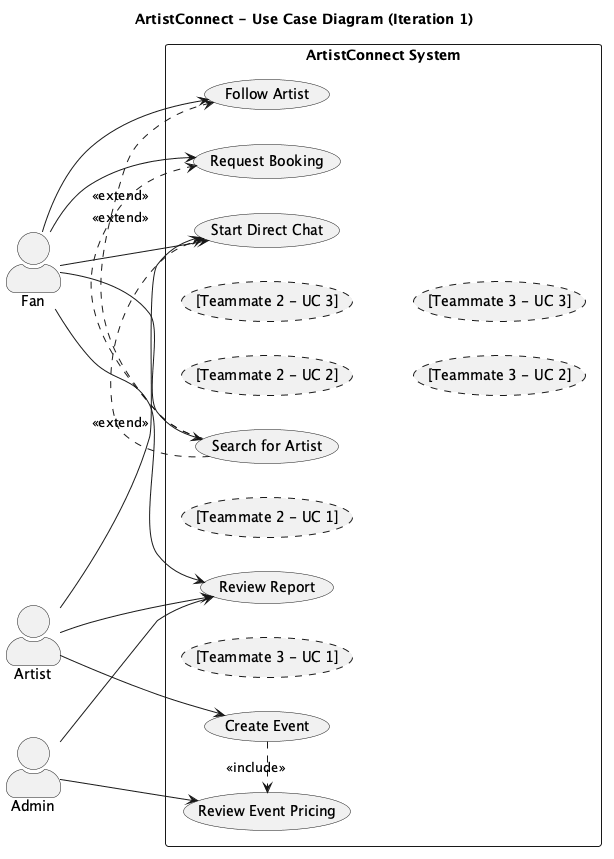
\includegraphics[width=\textwidth]{../use_case_diagram.png}
\end{center}

\fillin{This diagram currently shows only Alejandro's 3 use cases plus
placeholder ovals for teammates. Regenerate
\texttt{use\_case\_diagram.puml} (PlantUML source included alongside
this document) once every member's use cases are finalized, replacing
each dashed placeholder oval with the real use case name and its
correct actor associations.}

% ============================================================
\chapter{System Sequence Diagram}

\begin{guidance}[Consistency with use cases]
Every scenario shown here should correspond to a use case described
earlier, using the same name. Missing or renamed scenarios break
traceability between Use Cases and SSDs.
\end{guidance}

\section*{\fillin{Scenario Name}}
\fillin{Insert system sequence diagram here.}

\begin{longtable}{|p{0.48\textwidth}|p{0.48\textwidth}|}
\hline
\textbf{Actor} & \textbf{System} \\
\hline
1. \fillin{step} & \\
\hline
 & 2. *\fillin{system response} \\
\hline
3. \fillin{step} & \\
\hline
\end{longtable}

\bigskip
\textit{Repeat for each scenario.}

% ============================================================
\chapter{Domain Model}

\begin{guidance}[Domain model is not a class diagram]
Use only nouns from the problem statement as domain classes. Do not
include methods, data types, UI classes, or persistence/database
details -- those belong to design, not analysis. Show entities and the
associations/multiplicities between them, not implementation.
\end{guidance}

\fillin{Insert domain model diagram here, e.g.\\
\texttt{\textbackslash includegraphics[width=\textbackslash textwidth]\{domain\_model.png\}}}

% ============================================================
\chapter{Operation Contracts}

\begin{guidance}[One contract per key system operation]
An operation contract documents \emph{what} a system operation
guarantees, not \emph{how} it is implemented. Postconditions describe
instances created/deleted, associations formed/broken, and attributes
changed -- written in the past tense, as if describing what has already
happened. Write one contract per team member's use cases (typically the
one system operation in the main success scenario that changes state).
\end{guidance}

\section*{Operation: searchArtists(criteria: SearchCriteria): List\textlangle ArtistSummary\textrangle}
\begin{description}[leftmargin=2.8cm, style=nextline]
  \item[Cross Reference] UC: Search for Artist -- Fan
  \item[Preconditions]
    \begin{itemize}
      \item The Fan is logged into the system.
    \end{itemize}
  \item[Postconditions]
    \begin{itemize}
      \item A collection of Artist instances matching the given criteria (name, genre, location) was retrieved.
      \item No system state was created, modified, or deleted (read-only operation).
    \end{itemize}
\end{description}

\section*{Operation: resolveReport(reportId: ReportID, action: ActionType): void}
\begin{description}[leftmargin=2.8cm, style=nextline]
  \item[Cross Reference] UC: Review Report -- Admin
  \item[Preconditions]
    \begin{itemize}
      \item The Admin is logged in with administrative privileges.
      \item A Report instance identified by \texttt{reportId} exists with status = "Pending."
    \end{itemize}
  \item[Postconditions]
    \begin{itemize}
      \item The Report instance's \texttt{status} attribute was changed to "Resolved."
      \item A new Resolution instance was created and associated with the Report, recording the acting Admin, the action taken, and a timestamp.
      \item If \texttt{action} = DeleteContent, the associated Message, Profile, or Event instance's \texttt{status} attribute was changed to "Removed."
      \item If \texttt{action} = Suspend or Ban, the reported User instance's \texttt{status} attribute was changed to "Suspended" or "Banned" respectively.
      \item A new Notification instance was created and associated with the reporting User.
      \item A new Notification instance was created and associated with the reported User, if \texttt{action} $\neq$ Dismiss.
    \end{itemize}
\end{description}

\section*{Operation: submitEvent(eventData: EventForm): Event}
\begin{description}[leftmargin=2.8cm, style=nextline]
  \item[Cross Reference] UC: Create Event -- Artist
  \item[Preconditions]
    \begin{itemize}
      \item The Artist is logged in and owns an account in good standing.
    \end{itemize}
  \item[Postconditions]
    \begin{itemize}
      \item A new Event instance was created with \texttt{title}, \texttt{dateTime}, \texttt{location}, \texttt{description}, \texttt{capacity}, and \texttt{proposedPrices} set from \texttt{eventData}.
      \item The new Event instance's \texttt{status} attribute was set to "Pending Approval."
      \item An association was formed between the new Event instance and the Artist who created it.
      \item The new Event instance was added to the Admin approval queue.
    \end{itemize}
\end{description}

\bigskip
\textit{Repeat the operation contract pattern above for each additional team member's key use-case operation.}

% ============================================================
\chapter{Test Cases}

\begin{guidance}[Traceability of tests]
Each test case should reference the requirement or use case it
verifies. Keep test case IDs consistent across iterations so gaps in
coverage are easy to spot.
\end{guidance}

\section{Test Cases for Iteration 1}

\textbf{Target Users:} \fillin{Who}

\textbf{What is covered in the tests:}
\begin{enumerate}
  \item \fillin{Area of functionality covered}
\end{enumerate}

\subsection*{Test Case: \fillin{ID, e.g., T1}}
\begin{itemize}
  \item \textbf{Description:} \fillin{What this test checks}
  \item \textbf{Action:} \fillin{Function/action exercised}
  \item \textbf{Related Requirements:} \fillin{Preconditions}
  \item \textbf{Expected Result:} \fillin{Expected behavior}
  \item \textbf{Test Result:} \fillin{Actual behavior observed}
  \item \textbf{Status:} \fillin{Pass / Fail}
\end{itemize}

\bigskip
\textit{Repeat the Test Case block above for each test in this iteration.}

\section{Test Cases for Iteration 2}
\fillin{Same structure as Iteration 1.}

\section{Test Cases for Iteration 3}
\fillin{Same structure as Iteration 1.}

\section{Test Cases for Final Iteration}
\fillin{Same structure as Iteration 1.}

\end{document}
